%!TEX root = ../main.tex
\subsection{Node Software}
An example of a node can be seen in figure \ref{fig:gps_node}.

\begin{figure}[!h]
\centering
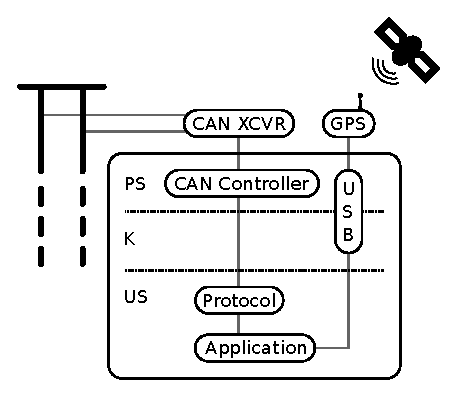
\includegraphics[width=0.5\textwidth]{graphics/analysis_gps.eps}
\caption{GPS node implemented on Zybo board.}
\label{fig:gps_node}
\end{figure}

This specific node has a GPS attached to it connected through a USB interface, but in general it could be any kind of data producing unit connected through any kind of interface.
From the analysis section is it clear that a node has the following responsibilities:

\begin{itemize}
\item Get data from associated sensor.
\item Pack data according to the specified protocol.
\item Construct CAN package
\item Send data using a CAN controller.
\item Get data from CAN network.
\item React to commands sent to it.
\end{itemize}

A node can be any kind of microcontroller, but this section will only address the case where a Zybo board is used as node microcontroller. 
The requirements state that it should be simple to add nodes to the system. 
To realize this the node software should be designed to be modular.
It should be easily identified what software and what interface a developer of a new node must adhere to.
The coming sections will explain the design of the node software that will provide the mentioned functionality using the design requirements.

The first section will explain the software running on the userspace in Linux, whereas the next section will address the use of the built in CAN controller.	

\subsubsection*{Userspace Software}
To design modular software it needs to be analyzed which responsibilities are the same for all nodes and which are sensor specific.
The sensor specific tasks are found to be getting data from sensor and to pack data according to the specified protocol.
The remaining responsibilities are the same for all nodes in the system. 
A class diagram showing the designed software can be seen in figure \ref{fig:node_class_diagram}.
Classes to the right of the dashed horizontal is sensor specific and should be developed for each specific sensor.
Classes to the left are agnostic to all data they receive going from the sensor and to the CAN network.
They are generic classes and should be reused when developing new nodes.
The classes and their functionalities will be explained.


\begin{lstlisting}[caption=Struct for data packet.,label=code:data_packet]
struct data_packet {
  std::bitset<1> sof;
  std::bitset<4> node_id;
  std::bitset<4> n_data_bytes;
  std::bitset<6> messagetype;
  std::vector<bool> data;
(*@\makebox[\linewidth][c]{$\smash{\vdots}$}@*)
};
\end{lstlisting}


~\\ \par \textbf{GPS class} ~ \\
The GPS class needs to get data from a connected GPS unit and update its own variables with that data.
The specific GPS unit used in this project has a USB interface and uses the NMEA protocol to format data.
Whenever its variables has been updated with new data it calls xxxfunction from the Packer\_GPS.

~\\ \par \textbf{Packer\_GPS class} ~ \\
The Packer\_GPS class is also sensor specific and is the link between the sensor and the data agnostic node.
It is hard-coded with the message types that the sensor is allowed to send onto the network.
It has the responsibility to acquire data from the sensor class and pack it according to the developed protocol.
The reason for making a separate class for the packer and not putting the functionality into the GPS class is that if the specification of the protocol or message types change, only this class needs to be modified.

~\\ \par \textbf{Node class} ~ \\
The class has knowledge about node id and appends it to all data packets that are passed to it.
The class has the responsibility of keeping track of milliseconds since last received synchronize message.
It needs to create a time message each time data is to be sent.
The class receives start, stop or synchronize events from the protocol class and reacts to those accordingly.

~\\ \par \textbf{Protocol class} ~ \\
The protocol cla

\begin{figure}[!h]
\centering
\missingfigure[figwidth=1\textwidth]{Class diagram}
\caption{Class diagram showing node software.}
\label{fig:node_class_diagram}
\end{figure}


\subsubsection*{CAN Controller Software}
\mikkel{Catalins stuff should be here?}